\documentclass[12pt,a4paper,titlepage]{article}
\usepackage{lab_style}
\usepackage{pdfpages}
\usepackage{eso-pic}
\usepackage{graphicx}
\usepackage{float}
\newcommand\tab[1][1cm]{\hspace*{#1}}

\graphicspath{ {./} }
  
\begin{document}

\begin{titlepage}
\selectlanguage{english}

%----------------------------------------------------------------------------------------
% TITLE PAGE INFORMATION
%----------------------------------------------------------------------------------------
  \begin{center} % Center everything on the page

  %----------------------------------------------------------------------------------------
  % HEADING SECTIONS
  %----------------------------------------------------------------------------------------
  \textsc{\large Faculty of Computers, Informatics and Microelectronics}\\[0.5cm]
  \textsc{\large Technical University of Moldova}\\[1.2cm] % Name of your university/college
  \vspace{25 mm}

  \textsc{\Large Object-Oriented Modeling and Analysis}\\[0.5cm] % Major heading such as course name
  \textsc{\large Laboratory work \#8}\\[0.5cm] % Minor heading such as course title

\newcommand{\HRule}{\rule{\linewidth}{0.5mm}} % Defines a new command for the horizontal lines, change thickness here

  %----------------------------------------------------------------------------------------
  % TITLE SECTION
  %----------------------------------------------------------------------------------------
  \vspace{10 mm}
  \HRule \\[0.4cm]
  { \LARGE \bfseries Modeling your project with Component Diagrams. Project setup. Top-down and bottom-up
design. }\\[0.4cm] % Title of your document
  \HRule \\[1.5cm]

  %----------------------------------------------------------------------------------------
  % AUTHOR SECTION
  %----------------------------------------------------------------------------------------
      \vspace{30mm}

      \begin{minipage}{0.4\textwidth}
      \begin{flushleft} \large
      \emph{Author:}\\
      Cernei \textsc{Liviu}
      \end{flushleft}
      \end{minipage}
      ~
      \begin{minipage}{0.4\textwidth}
      \begin{flushright} \large
      \emph{Supervisor:} \\
      Mihail \textsc{Gavrilița} % Supervisor's Name
      \end{flushright}
      \end{minipage}\\[4cm]

      \vspace{5 mm}
      % If you don't want a supervisor, uncomment the two lines below and remove the section above
      %\Large \emph{Author:}\\
      %John \textsc{Smith}\\[3cm] % Your name

      %----------------------------------------------------------------------------------------
      % DATE SECTION
      %----------------------------------------------------------------------------------------

      {\large Chișinau 2018}\\[3cm] % Date, change the \today to a set date if you want to be precise

      %----------------------------------------------------------------------------------------
      % LOGO SECTION
      %----------------------------------------------------------------------------------------

      %\includegraphics{red}\\[0.5cm] % Include a department/university logo - this will require the graphicx package

      %----------------------------------------------------------------------------------------

      \vfill % Fill the rest of the page with whitespace
      \end{center}
      
\end{titlepage}

\cleardoublepage

\newpage

\pagenumbering{arabic}
\setcounter{page}{1}
\setcounter{secnumdepth}{4}

\addtocontents{toc}{\protect\thispagestyle{empty}} % no page number on the table of contents page
\cleardoublepage


\phantomsection
\addcontentsline{toc}{section}{Introduction}
\section*{Laboratory work \#8}
\phantomsection

\section{Tasks}
\begin{itemize}
	\item
	Model your application using 3 Component Diagrams;
	\item 
	Describe the steps needed to setup your project.
\end{itemize}

\section{Theory}

\subsection{Top-down and Bottom-up Design}
Top-down and bottom-up are both strategies of information processing and knowledge ordering, used in a variety of fields including software, humanistic and scientific theories (see systemics), and management and organization. In practice, they can be seen as a style of thinking, teaching, or leadership.\par
A top-down approach (also known as stepwise design and in some cases used as a synonym of decomposition) is essentially the breaking down of a system to gain insight into its compositional sub-systems in a reverse engineering fashion. In a top-down approach an overview of the system is formulated, specifying, but not detailing, any first-level subsystems. Each subsystem is then refined in yet greater detail, sometimes in many additional subsystem levels, until the entire specification is reduced to base elements. A top-down model is often specified with the assistance of "black boxes", which makes it easier to manipulate. However, black boxes may fail to clarify elementary mechanisms or be detailed enough to realistically validate the model. Top down approach starts with the big picture. It breaks down from there into smaller segments.\par
A bottom-up approach is the piecing together of systems to give rise to more complex systems, thus making the original systems sub-systems of the emergent system. Bottom-up processing is a type of information processing based on incoming data from the environment to form a perception. From a cognitive psychology perspective, information enters the eyes in one direction (sensory input, or the "bottom"), and is then turned into an image by the brain that can be interpreted and recognized as a perception (output that is "built up" from processing to final cognition). In a bottom-up approach the individual base elements of the system are first specified in great detail. These elements are then linked together to form larger subsystems, which then in turn are linked, sometimes in many levels, until a complete top-level system is formed. This strategy often resembles a "seed" model, by which the beginnings are small but eventually grow in complexity and completeness. However, "organic strategies" may result in a tangle of elements and subsystems, developed in isolation and subject to local optimization as opposed to meeting a global purpose.\par
\clearpage

\section{Component Diagrams}
In Figure ~\ref{fig:intermediar} is represented the component diagram for app, using the MVC pattern.
\begin{figure}[H]
\centering
	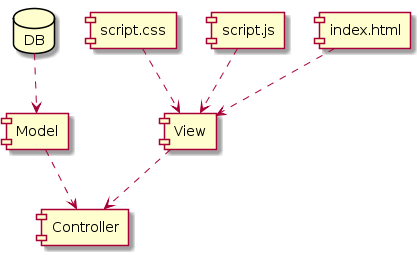
\includegraphics[width=10cm]{intermediar}
	\caption{MVC component diagram}
	\label{fig:intermediar}
\end{figure}

In Figure ~\ref{fig:final} is represented the component diagram for the app, after compiling, minifiing scripts.
\begin{figure}[H]
\centering
	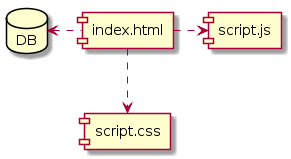
\includegraphics[width=10cm]{final}
	\caption{Compiled files component diagram}
	\label{fig:final}
\end{figure}

\section{Project Setup}
The last step of website development is deployment. The process of“getting your website on the web” consists of a number of steps:

\begin{itemize}
	\item
	Finding a domain name
\item
	Finding a hosting service
\item
	Uploading files with SFTP
	\item 
	Deploying server-side applications
\end{itemize}

But the client is not required to download or install anything. He simply navigates to the webpage. The only step he should take is to create an account.

\section{Conclusion}
In this laboratory work we learned to create component diagrams and explain Project Setup.

\clearpage
\cleardoublepage

\end{document}
